%% Преамбула TeX-файла

% 1. Стиль и язык
\documentclass[utf8x, 12pt]{G7-32} % Стиль (по умолчанию будет 14pt)

% Остальные стандартные настройки убраны в preamble.inc.tex.
\include{preamble.inc}

% Настройки листингов.
\ifPDFTeX
\include{listings.inc}
\else
\usepackage{local-minted}
\usepackage{mdframed}
\fi

% Полезные макросы листингов.
\include{macros.inc}
\include{00-title}


\begin{document}

\frontmatter % выключает нумерацию ВСЕГО; здесь начинаются ненумерованные главы: реферат, введение, глоссарий, сокращения и прочее.

\begin{titlepage}

\end{titlepage}

\begin{executors}
\personalSignature{Первый исполнитель}{ФИО}

\personalSignature{Второй исполнитель}{ФИО}
\end{executors}

%\tableofcontents

%\listoffigures

%\listoftables

%\NormRefs % Нормативные ссылки 
% Команды \breakingbeforechapters и \nonbreakingbeforechapters
% управляют разрывом страницы перед главами.
% По-умолчанию страница разрывается.

% \nobreakingbeforechapters
% \breakingbeforechapters

\include{00-abstract}

\tableofcontents

%\Defines % Необходимые определения. Вряд ли понадобться
\begin{description}
\item[Распределённый] Слово, которое нельзя употреблять. Но надо протестировать длинные строки в глоссарии.
\item[JCR] Java Content Repository - java API to store data.
\item[OSGI] Open gateway initiative
\item[Replication] Process of copying content from Author instance to Publish instance
\item[Авторский сервер (Author instance)] Сервер, предназначенный для создания контента и управления им. Данный сервер предназначен для работы авторов(контент-менеджеров), которые использую удобный интуитивно понятный интерфейс занимаются наполнением контента сайта. 
\item[Публичный сервер (Publish instance)] Сервер делает контент, создаваемый авторами, доступным для целевой аудитории (пользователей).
\item[Репликация] Механизм в AEM используемый для публикации (копирования) контента с Авторского сервера на Публичный сервер.
\item[Bundle] модули в контексте OSGI спецификации. Представляет из себя jar файл с дополнительной мета информацией.
\end{description}

%%% Local Variables:
%%% mode: latex
%%% TeX-master: "rpz"
%%% End:

\Abbreviations %% Список обозначений и сокращений в тексте
\begin{description}
\item[AEM (Adobe experience manager)] Система управления контентом которая осуществляет обработку и доставку различных видов контента. Система реализована на языке Java с использованием большого количества фреймворков, но основой системы является фреймворк построения модульного приложения – OSGI.
\item[Фреймворк] программная платформа, определяющая структуру программной системы; программное обеспечение, облегчающее разработку и объединение разных компонентов большого программного проекта.
\item[JCR (Java content repository)] Тип объектной базы данных, используется в системе AEM для хранения, поиска и извлечения иерархических данных.
\item[OSGI] Cпецификация для построения модульных систем для платформы Java \cite{web:osgiSite}.
\item[Бандл (bundle)] модули в терминах OSGI спецификации. Представляет из себя JAR архив с дополнительной мета информацией.
\item[Лэндскейп (landscape)] Набор элементов аппаратного обеспечения, программного обеспечения и средств, расположенных в определенной конфигурации.
\item[Диспетчер (dispatcher)] Это средство кэширования и / или балансировки нагрузки в Adobe Experience Manager.
\item[Режимы работы (run modes)] Позволяют настраивать экземпляры AEM для конкретных целей и задавать базовую конфигурацию.
%\item[Авторский сервер (Author instance)] Сервер, предназначенный для создания контента и управления им. Данный сервер предназначен для работы авторов(контент-менеджеров), которые использую удобный интуитивно понятный интерфейс занимаются наполнением контента сайта.
\item[Экземпляр автора (Author instance)] Среда, предназначенная для создания контента и управления им. Основные пользователи авторы(контент-менеджеры).
\item[Экземпляр публикации (Publish instance)] Среда, предоставляющая пользователям доступ к контенту созданному авторами.
%\item[Публичный сервер (Publish instance)] Сервер делает контент, создаваемый авторами, доступным для целевой аудитории (пользователей).
\item[SSO (Single Sign-On)] Технология единого входа пользователей, с помощью которой пользователь проходит аутентификацию один раз и может посещать другие порталы, приложения и сайты без повторной аутентификации.
\item[SLO (Single Log-Out)] Технология единого выхода позволяет пользователю завершить сессии во всех приложениях установленные во время SSO, запустив процесс выхода из системы один раз.
\item[SAML (security assertion markup language)] Язык разметки, основанный на языке XML с помощью которого реализуется SSO и SLO. Является открытым стандартом обмена данными аутентификации и авторизации между участниками, в частности, между поставщиком учётных записей и поставщиком услуг.
\item[IdP (identity provider)] Поставщик учетных записей – центральный сервер который хранит аккаунты пользователей.
\item[SP (service provider)] Поставщик услуг – сервис на стороне приложения который обращается к IdP для авторизации пользователя.
\item[Привязка (SAML Binding)] Определяет порядок использования транспортных протоколов для передачи SAML сообщений между участниками.
\item[Утверждение (SAML Assertion)] XML Данные отправляемые поставщиком учетных записей поставщику услуг, которые содержат данные авторизации пользователя.
%Суть DS в том, что создается дескриптор сервиса: XML-файл, который описывает сервис. Затем данный файл регистрируется в манифесте бандла. Соответственно, OSGi-среда после ресолвинга зависимостей данного бандла автоматически стартует описанные сервисы и переводит бандл в состояние ACTIVE. Естественно, что активатор бандла при этом выполняется.
\end{description}

Определения связанные с архитектурой AEM более подробно рассмотрены в параграфе 3 главы 1.

%%% Local Variables:
%%% mode: latex
%%% TeX-master: "rpz"
%%% End:
 %Абривиатуры вручную, зачем?
%\renewcommand{\nomname}{Список сокращений} % строго перед \printnomenclature
%\printnomenclature % Автоматический список сокращений
%\nomenclature{УОСКВ}{Умственно-отсталый сферический конь в вакууме}

\Introduction

%КОММЕНТ ДО: где, для чего, кем используется система АЕМ. Какие есть проблемы с ней!
Adobe Experience Manager — система управления контентом, осуществляющая хранение, обработку и доставку различных видов контента, предназначенная для крупных компаний, имеющих потребности в управление быстро меняющимся контентом. Созданный контент публикуется на отдельных серверах, оптимизированных для быстрого и надежного чтения хранимых ресурсов. В компаниях использующих систему, может быть развернуто множество AEM сред, где каждая среда будет представлять из себя отдельный проект со своими уникальными модулями и контентом доступным конечным пользователям системы. 

Экземпляр автора системы имеет различные роли пользователей рассчитанные на контент-менеджеров и администраторов системы. Аккаунты пользователей хранятся внутри системе в JCR хранилище. Если в среде компании имеется поставщик учетных записей и имеется множество систем на базе AEM, содержащих контент доступный только авторизованным пользователям, то встроенная система ролей и пользователей не может быть использована. В таком случае экземпляры публикации должны выступать в роли поставщика услуг и взаимодействовать с поставщиком учетных записей для реализации технологии единого входа.

Целью данной работы является разработка модуля управления авторизацией системы AEM с использованием стандарта SAML \cite{web:wikiSaml}. Для достижения поставленной цели необходимо решить следующие задачи:

\begin{itemize}
\item Изучить механизмы доступные в системе AEM для реализации SSO и SLO. Сделать выводы о необходимости разработки нового функционала.
\item Изучить фреймворки реализующие стандарт SAML и их применимость в среде AEM, выбрать наиболее подходящий фремворк.
\item Разработать модуль реализующий SSO и SLO с использованием стандарта SAML и выбранного ранее фреймворка.
\item Проверить работоспособность разработанного модуля в среде компании на всех порталах и с развернутым поставщиком учетных записей.
\end{itemize}

В первой главе произведен обзор предметной области, сформулированы требования к разрабатываемому модулю, выбран фреймворк который будет использован при разработке модуля. Во второй главе приведены проектные решения с учетом выбранного в первой главе фреймворка. Третья глава описывает процесс разработки, тестирования модуля а также пользовательскую документацию.

\mainmatter % это включает нумерацию глав и секций в документе ниже

%Исследование
\chapter{Анализ предметной области}
\label{cha:analysis}
%
% % В начале раздела  можно напомнить его цель
%

%\textbf{//КОММЕНТАРИЙ:
%Формулировать задачу обязательно до обзора системы? Если знать архитектуру системы, тогда понятно как такие требования получаются...}

\section{Формулировка задачи}
Adobe Experience Manager — система управления контентом, осуществляющая хранение, обработку и доставку различных видов контента в масштабах предприятия. Система предназначена для крупных компаний, имеющих потребности в управление быстро меняющимся контентом, это могут быть как и внутренние корпоративные порталы так и порталы для внешних пользователей. Созданный контент публикуется на отдельных серверах, оптимизированных для быстрого и надежного чтения хранимых ресурсов.

Основные пользователи системы:
\begin{enumerate}
\item Авторы контента или контент-менеджеры - отвечают за наполнения сайтов контентом. В системе организована возможность удобного управления контентом портала, с использованием графического интуитивно понятного интерфейса, без перезагрузок и остановки работы портала, так как предполагается постоянное активное использование ресурсов пользователями. Авторам не требуются навыки программирования или разработки, и система предоставляет авторам следующие функции:
\begin{enumerate}
\item Возможность загружать в систему цифровые ресурсы, такие как картинки, видео, тексты и.др, 
\item Создавать страницы из шаблонов и редактировать существующие, наполнять страницы AEM компонентами и цифровыми ресурсами. 
\item Активировать созданный контент - т.е активировать процесс копирования ресурсов с сервера разработки на сервер публикации. 
\item Удалять не актуальный контент, в том числе и страницы или AEM компоненты и цифровые ресурсы с конкретных страниц. 
\item Копировать контент чтобы ускорить создание похожих ресурсов.
\end{enumerate}

\item Администратор - отвечает за развитие, поддержку работоспособности и безопасности системы. Для администратора предусмотрен графический веб-интерфейс отображающий информацию о состояние системы, компонентах и позволяющий производить настройку системы. Для работы администратора в системе предусмотрен следующий функционал:
\begin{enumerate}
\item Возможность загружать пакеты созданные разработчиками, или пакеты обновлений поставляемые разработчиками системы и устанавливать их. Пакеты могут содержать новые компоненты, шаблоны, цифровые ресурсы, файлы конфигураций, контент, модули системы. 
\item Возможность создавать пакеты с контентом - позволяет скачивать пакеты и переносить созданный контент на другие сервера с целью переиспользования уже созданного контента. 
\item Добавлять в систему новые модули, а так-же активировать, останавливать или удалять существующие. 
\item Останавливать, активировать и конфигурировать сервис-компоненты системы. 
\item Добавлять или удалять пользователей, группы пользователей, устанавливать права доступа. 
\item Выполнять тестирование системы по заданным стандартным параметрам, проводить диагностику отслеживать логи и состояние системы используя встроенные механизмы с заданными параметрами.
\end{enumerate}
\item Разработчик - Разработчики работающие с системой занимаются разработкой новых компонентов, шаблонов, и функционала системы. Для них также предусмотрена графическая веб-среда разработки. Архитектора позволяет разработчикам встраивать в систему новый функционал без необходимости останавливать работу системы и не нарушая работу других компонентов.
\end{enumerate}

Функционал предоставляемый системой полностью удовлетворяет потребности авторов контента а архитектура системы позволяет разработчикам легко разрабатывать и новый функционал для системы.

В компаниях использующих AEM может быть развернуто множество так называемых Лэндскейпов - Наборов элементов аппаратного обеспечения, программного обеспечения и средств, расположенных в определенной конфигурации. Лэндскейпы включают в себя различные наборы серверов в том числе с развернутыми на них AEM средами содержащими экземпляры авторов, публикации и диспетчеры (Приложение A рис.~\ref{fig:complexDeploy}). Каждая AEM среда представляет из себя отдельный проект со своими уникальными модулями и контентом, над которыми ведется активная разработка и внедряются новые модули со своими конфигурациями. Хотя в AEM и имеются механизмы для отслеживания состояния системы и её модулей и компонентов, они проверяют лишь основные параметры системы, и не имеют необходимых конфигураций для более тонкой настройки проверки. 

Вывод:
Исходя из вышеописанных пунктов возникла необходимость разработки модуля, расширяющего возможности мониторинга состояния системы, с возможностью задавать настройки проверок. Требуется отслеживать следующие показатели и информировать администратора в случае сбоев на любом из серверов:
\begin{itemize} 
\item Необходимо проверять механизмы копирования контента с экземпляров авторов на экземпляры публикации.
\item Необходимо проверять работоспособность модулей и их сервис-компонентов имеющих важное значение для работоспособности системы, и/или определенного функционала системы.
\item Проверять что режимы работы системы соответствует требуемым. 
\item Проверять доступность удаленных ресурсов от которых может зависеть работоспособность модулей и компонентов системы.
\item Предусмотреть возможность интеграции результатов проверок с программой мониторинга Nagios \cite{web:nagiosDocs}, для автоматического отслеживания их статуса и оповещения администратора в случае неисправностей.
\end{itemize}
% Обратите внимание, что включается не ../dia/..., а inc/dia/...
% В Makefile есть соответствующее правило для inc/dia/*.pdf, которое
% берет исходные файлы из ../dia в этом случае.

%\begin{figure}
%  \centering
%  \includegraphics[width=\textwidth]{inc/dia/rpz-idef0}
%  \caption{Рисунок}
%  \label{fig:fig01}
%\end{figure}
%
%В \cite{Pup09} указано, что...
%
%Кстати, про картинки. Во-первых, для фигур следует использовать \texttt{[ht]}. Если и после этого картинки вставляются <<не по ГОСТ>>, т.е. слишком далеко от места ссылки,~--- значит у вас в РПЗ \textbf{слишком мало текста}! Хотя и ужасный параметр \texttt{!ht} у окружения \texttt{figure} тоже никто не отменял, только при его использовании документ получается страшный, как в ворде, поэтому просьба так не делать по возможности.

\section{Обзор системы и используемых компонентов}

AEM – система построенная с использованием технологии Java. В основе системы лежит фреймворк OSGI.

\subsection{Архитектура OSGI}
OSGI – фреймворк для построения модульной, динамической системы в котором модуль называется бандл. Фреймворк имеет свой контекст, в который и устанавливаются все модули, они взаимодействуют между собой по средствам сервисов зарегистрированных в регистре сервисов рис.~\ref{fig:servicePattern}. Под динамической системой понимается возможность устанавливать, удалять и обновлять модули без перезапуска системы.

\begin{figure}[h]
  \centering
  \includegraphics[width=\textwidth]{inc/svg/servicePattern}
  \caption{Диаграмма архитектуры OSGI}
  \label{fig:servicePattern}
\end{figure}

OSGI спецификация концептуально разделяется на 3 уровня \cite{osgiInAction}:
\begin{enumerate}
\item Модульный уровень – уровень модулей, которые в терминах спецификации называются бандл (далее по тексту - модуль). Они представляют из себя JAR-архив с специальной мета-информацией. Модули содержат в себе java-классы и ресурсы. Модули могут реализовывать функционал системы, а так-же предоставлять сервисы для использования другими модулями. Дополнительная информация указывается в файле META-INF/MANIFEST.MF может иметь различные заголовки, ключевыми являются:
\begin{itemize}
\item Bundle-Name - имя модуля.
\item Bundle-SymbolicName - символьное имя, которое однозначно идентифицирует модуль.
\item Bundle-Version - указывает версию модуля.
\item Import-Package - заголовок указывает внешние зависимости модуля (импортируемые Java-пакеты из других модулей). Могут быть указаны конкретные версии или диапазоны версий для каждой зависимости.
\item Export-Package - заголовок указывает java-пакеты, которые видны вне модуля. Если пакет не объявлен в этом заголовке, он будет виден только внутри модуля.
\item Bundle-Activator - имя класса в котором заданы действия выполняющиеся при запуске модуля.
\item Service-Component - заголовок содержащий список XML-файлов описывающих сервис-компоненты модуля.
\end{itemize}

\item Уровень жизненного цикла – уровень, определяющий, и управляющий операциями жизненного цикла модулей, состоит из нескольких состояний. Жизненным циклом модуля управляет OSGI контейнер (рис.~\ref{fig:bundleLifeCycle}).

Этапы жизненного цикла модулей в OSGI:
\begin{itemize}
\item INSTALLED - модуль успешно установлен в систему.
\item RESOLVED - модулю доступны все необходимые зависимости и он готов к запуску.
\item STARTING - выполняются действия запуска модуля описанные в активаторе.
\item ACTIVE - модуль успешно запущен.
\item STOPPING - выполняются действия остановки модуля.
\item UNINSTALLED - модуль удален, означает завершение жизненного цикла модуля.
\end{itemize}

\begin{figure}
  \centering
  \includegraphics[width=\textwidth]{inc/svg/LifeCycle}
  \caption{Возможные состояния модуля в OSGI}
  \label{fig:bundleLifeCycle}
\end{figure}

\item Уровень сервисов - позволяет модулям взаимодействовать между собой с помощью сервисов. Во время запуска модули регистрируют объекты с реализацией заявленного интерфейса в регистре сервисов OSGI фреймворка (Приложение А рис.~\ref{fig:simpleServices}). Другие модули могут находить и использовать зарегистрированные сервисы. Другим подходом к регистрации сервисов являются декларативные сервисы - Суть декларативных сервисов заключается в том, что создается дескриптор сервиса: XML-файл, который описывает сервис. Затем данный файл регистрируется в MANIFEST файле модуля. Диаграмма жизненного цикла декларативных сервисов приведена в Приложении A рис.~\ref{fig:declareService}.

\end{enumerate}

\subsection{Архитектура AEM}
Основу AEM составляют набор модулей, которые можно условно выделить в 4 компоненты:
\begin{enumerate}
\item Java content repository – один из типов объектной базы данных, созданных для хранения и извлечения иерархических данных. Данные в JCR представляют из собой дерево, состоящее из узлов с ассоциированными с ними свойствами. Эти свойства и являются хранимыми данными, и могут хранить строки, числа или основные примитивные типы данных, а так-же двоичные данные, изображения и.т.д. 
\item Apache Sling – веб-фреймворк построенный по архитектуре REST, отвечающий за доставку контента в контент-ориентированных приложениях с использованием JCR.
\item AEM модули – набор бандлов реализованных компанией Adobe с использованием вышеупомянутых технологий.
\item Пользовательские модули – модули, разрабатываемые разработчиками, и расширяющие функционал системы.
\end{enumerate}

\begin{figure}[h]
  \centering
  \includegraphics[width=\textwidth]{inc/dia/osgi}
  \caption{Архитектура AEM}
  \label{fig:fig02}
\end{figure}

%\textbf{//Комментарий: Если дальше буду говорить про какие-то фишки системы которые проверяю, т.е РЕПЛИКАЦИЯ, Режимы запуска, Жизненный цикл компонентов, то их тоже нужно тут указать?}


%Выделить какой-то абзац под описание ключевых фишек(компонентов) AEM
AEM - серверное приложение, работающее на платформе Java. Оно доступно в виде исполняемого JAR файла (файл быстрого запуска). Установка приложения создаст экземпляр который может быть либо экземпляром автора либо публикации, что задается режимом запуска. В разработке используется несколько развернутых сред.
\begin{itemize}
\item Среда разработки - используется разработчиками для разработки новых модулей системы. Может состоять как из экземпляров авторов и публикации, так и только иметь экземпляр автора, в таком случае тестирование сразу проводится в тестовой среде.
\item Среда тестирования - тестовая среда в которой проверяется функционал разработанных модулей и дизайн шаблонов, компонентов и ресурсов.
\item Рабочая среда - среда состоящая из экземпляров авторов и публикации. Где авторы вносят актуальный контент в экземпляры публикации а пользователи имеют доступ к контенту через экземпляры публикации. Как правило в рабочей среде используется несколько раздельных серверов с развернутыми на них экземплярами публикации и их работой управляет диспетчер осуществляющий кэширование и распределение нагрузки между серверами.
\end{itemize}

Экземпляр - В терминологии AEM экземпляр является копией AEM, запущенной на сервере. Установленные экземпляры отличаются своими конфигурациями. Конфигурации задаются с помощью режимов работы, выделяют два основных типа экземпляров AEM:
\begin{itemize}
\item Авторский экземпляр - экземпляр как правило расположенный за внутренним фаерволом и предназначен для работы авторов контента. 
\item Экземпляр публикации - как правило располагаются на общедоступных серверах через которые посетители могут иметь доступ к сайту и взаимодействовать с ним.
\end{itemize}

Режим работы - Режимы работы позволяют настраивать экземпляр AEM для конкретной цели. Например, как экземпляры автора или публикации, тестирования, разработки или другие. Режимы работы позволяют задать параметры конфигурации системы и дополнительные модули которые необходимо установить при установки экземпляра. Режимы запуска делятся на 2 типа:
\begin{itemize}
\item Установочные - задаются в момент установки экземпляра, и их нельзя поменять при последующих перезапусках. К таким режимам относят:
\begin{enumerate}
\item author - определяет конфигурации для экземпляра автора (взаимоисключающий с publish)
\item publish - определяет конфигурации для экземпляра публикации (взаимоисключающий с author) 
\item samplecontent - установка пакетов с демонстрационных контентом (используется для тестирования и разработки, взаимоисключающий с nosamplecontent)
\item nosamplecontent - пустой экземпляр без дополнительного контента (используется для рабочих экземпляров, взаимоисключающий с samplecontent)
\end{enumerate}
\item Пользовательские - режимы запуска созданные пользователями. Они задают необходимые параметры конфигурации системы и модули которые необходимо установить. Эти режимы можно менять при каждом запуске экземпляра.
\end{itemize}

Репликация - процесс копирования контента с экземпляров автора на экземпляры публикации. Во время активации контента автором вручную, или по расписанию создается пакет, который потом копируется на экземпляр публикации и устанавливается. Для задания правил копирования, расписания и экземпляров на которые осуществляется копирование используются конфигурации которые называются агентами репликации.

\subsection{Обзор используемых модулей}
	В системе имеется механизм для отслеживания некоторых параметров и состояний - модули "Apache Sling Health Check Core" и "Apache Sling Health Check Web Console Plugin". С их помощью реализуется функционал выявления ошибок в системе и администратору предоставляется веб интерфейс управления функционалом выявления ошибок соответственно \cite{web:slingHealthCheck}.

Модуль "Apache Sling Health Check Web Console Plugin"
	С помощью этого модуля реализован интерфейс для администратора, в котором он может настроить параметры проверок, и осуществляется вывод результата проверок в веб-консоли. В веб интерфейсе можно задавать следующие параметры:
\begin{itemize}
\item Health Check tags - Список тэгов по которым будет отобраны проверки для выполнения.
\item Combine tags with logical 'OR' - Выбирать проверки с любым тэгом из списка тэгов.
\item Show DEBUG logs - Показывать дебаг логи.
\item Show failed checks only - Отображать только проверки с ошибками.
\item Override global timeout - Переопределить глобальное максимальное время выполнения проверки.
\end{itemize}

Модуль "Apache Sling Health Check Core"
	С помощью данного модуля в системе реализован функционал осуществляющий выполнение сервисов, позволяющих администратору определить наличие ошибок в системе, а в некоторых случаях и определить их причины. Модуль регистрирует в системе набор настроенных проверок. Для каждой проверки создается JMX MBean предоставляющий доступ к логу выполнения и результату. Также этот модуль предоставляет интерфейс позволяющий расширять функционал системы пользовательскими проверками. 
	 
	В результате анализа модуля "Apache Sling Health Check Core" были выявлены 3 проверки наиболее соответствующие заданным требованиям.
	
	Обзор имеющихся проверок приведен в таблице 1.1
		
\begin{table}[ht]
  \caption{Сравнение SAML \cite{web:wikiSaml} фреймворков}
  \begin{tabular}{|p{3cm}|p{47mm}|p{30mm}|p{35mm}|}
  \hline
  Название      
  & Поддержка 
  & Количество запросов на stackoverflow 
  & Примеры \\
  \hline
  OpenSAML 3  
  & Поддерживается, последняя версия: март 2017
  & 399
  & Есть примеры, книги \\
  \hline
  OneLogin       			   
  & Поддерживается, последняя версия: ноябрь 2018
  & 324
  & Есть примеры \\
  \hline
  Spring Security SAML                
  & Поддерживается, последняя версия: март 2019
  & боле 500
  & Есть примеры \\
  \hline
  Pac4j       			   
  & Поддерживается, последняя версия: февраль 2019
  & 16
  & Есть примеры \\
  \hline
  \end{tabular}
  \label{tab:tabular}
\end{table}	
	
	Обнаруженные проверки не могут удовлетворить потребности в полном объеме.
\begin{enumerate}
\item Replication and Transport Users - Не имеет конфигурации, а следовательно не выполняет требуемых проверок.
\item Active Bundles - Наиболее подходящая проверка, но выполняет избыточную проверку, необходимо проверять только заданные модули, проверка всех модулей может привести к ложным срабатываниям и не осуществляет проверку статуса компонент.
\item Replication Queue - Осуществляет проверку очереди, но не размер очереди, а количество попыток первого элемента, так-же нет конфигурации для проверки активных и неактивных агентов репликации.
\end{enumerate}

Вывод: Стандартные модули системы не позволяют реализовать требуемый функционал в полном объеме. Система предоставляет интерфейс с помощью которого можно расширить функционал проверок системы.

\section{Формальные требования}


%ПРОВЕРКА АГЕНТОВ РЕПЛИКАЦИИ
\subsection{Проверка агентов репликации}
Осуществляет проверку наличия в системе всех сконфигурированных агентов репликации, их состояние, размер их очереди, и для активных агентов, с не переполненной очередью, выполняет тестовую репликацию. Наличие в системе активных агентов которые не проверяются и не игнорируются приведет к провалу проверки.

Требуемые параметры конфигурации:
\begin{itemize}
\item Имена агентов репликации наличие и состояние которых необходимо проверить.
\item Имена агентов репликации которые игнорируются во время проверки.
\item Максимально разрешенный размер очереди для агентов.
\end{itemize}
%END REPLICATION AGENTS

%APPLICATION BUNDLE CHECK
\subsection{Проверка модулей конкретных приложений}
Осуществляет проверку наличия в системе всех перечисленных в конфигурации модулей, проверяет что они активны, и выполняет проверку активности и статуса всех сервис-компонент входящих в этот модуль.

Требуемые параметры конфигурации:
\begin{itemize}
\item Список полных символьных имен модулей, статус которых необходимо проверить.
\item Список имен компонентов, которые должны быть отключены.
\end{itemize}
%END APPLICATION BUNDLE CHECK

%PING HEALTH CHECK
\subsection{Проверка доступности удаленных ресурсов}
Осуществляет проверку доступности удаленных ресурсов заданных в конфигурации с помощью URL.

Требуемые параметры конфигурации:
\begin{itemize}
\item Список HTTP URL систем доступность которых требуется проверить.
\end{itemize}
%PING HEALTH CHECK END

%RUN MODES HEALTH CHECK
\subsection{Проверка режимов работы}
Осуществляет проверку соответствия режимов работы системы и режимов из конфигурации проверки. Только полное соответствие допустимо.

Требуемые параметры конфигурации:
\begin{itemize}
\item Список режимов работы которым должен соответствовать экземпляр
\end{itemize}
%END RUN MODES HEALTH CHECK

%NAGIOS INTEGRATION
\subsection{Интеграция с Nagios}
Предусмотреть возможность интеграции проверок с программой Nagios: Программа должна периодически опрашивать проверки и получать их статус и лог выполнения проверок, статус сервиса в Nagios должен соответствовать статусу проверки, в случае сбоя администратору должно отправляться оповещение по электронной почте.
%END NAGIOS INTEGRATION

\section{Заключение}
В данной главе был произведен обзор системы и рассмотрены сценарии развертывания при которых возникает необходимость разработки пакета, расширяющего возможности мониторинга состояния системы. Встроенные механизмы мониторинга не имеют необходимых настроек чтобы покрыть требования заказчика, но предоставляют возможность расширения функционала мониторинга системы. Было принято решение разработать пакет расширяющий стандартный функционал мониторинга системы и реализовать интеграцию с системой мониторинга Nagios.


%%% Local Variables:
%%% mode: latex
%%% TeX-master: "rpz"
%%% End:

%Постановка задачи и проектирование
\chapter{Проектирование}
\label{cha:design}

%В данном разделе реализуется новая всячина.
При разработки нового модуля было решено использовать существующие фреймворки, реализующие стандарт SAML. В данной главе приведен обзор выбранных фреймворков и произведен анализ возможности их интеграции с системой AEM. На основе выбранного фреймворка спроектирована архитектура разрабатываемого модуля. 

\section{Выбор фреймворка}
Список фреймворков, рассматриваемых при разработке, был получен с официального сайта SAML \cite{web:samlFrameworksOasis} и со страницы в википедии \cite{web:samlFrameworksWiki}. Поскольку AEM основана на Java были выбраны только совместимые с системой фреймворки. 

\subsection{Обзор выбранных фреймворков}
Для сравнения выбранных фреймворков была составлена таблица 2.1, в которой выполняется сравнение по следующим параметрам:

\begin{itemize}
\item Поддержка - осуществляется ли поддержка библиотеки, когда выпущена последняя версия.
\item Количество запросов на stackoverflow - количество запросов на stackoverflow показывает насколько популярна библиотека.
\item Примеры и документация - наличие примеров и документации.
\end{itemize}

\begin{longtable}{|p{3cm}|p{47mm}|p{30mm}|p{35mm}|}
  \caption{Сравнение SAML фреймворков}
  \label{tab:tabular}
  \\ \hline
  Название & Поддержка & Количество запросов на stackoverflow & Примеры и документация \\
  \hline \endfirsthead
  \subcaption{Продолжение таблицы~\ref{tab:tabular}}
  \\ \hline \endhead
  \hline \subcaption{Продолжение на след. стр.}
  \endfoot
  \hline \endlastfoot
  Название      
  & Поддержка 
  & Количество запросов на stackoverflow 
  & Примеры и документация \\
  \hline
  OpenSAML 3  
  & Поддерживается, последняя версия: март 2017
  & 399
  & Есть примеры, книги, плохая документация на официальном сайте \\
  \hline
  OneLogin       			   
  & Поддерживается, последняя версия: ноябрь 2018
  & 324
  & Есть примеры, хорошая документация на официальном сайте \\
  \hline
  Spring Security SAML                
  & Поддерживается, последняя версия: март 2019
  & боле 500
  & Есть примеры, плохая документация на официальном сайте \\
  \hline
  Pac4j       			   
  & Поддерживается, последняя версия: февраль 2019
  & 16
  & Есть примеры, хорошая документация на официальном сайте \\
  \hline
\end{longtable}	

Составленная таблица не позволяет однозначно сказать какое решение подойдет лучше всего, поэтому с использованием каждого фреймворка был разработан прототип приложения, формирующий сообщение авторизации с заданным параметрами-заглушками, пример сообщения приведен в листинге \ref{lst:authnRequestExample}. Разработанные прототипы позволят сравнить возможности настройки фреймворков, удобство использования и доработок под свои нужны.

\begin{longlisting}
\inputminted[linenos,frame=single]{xml}{inc/src/authnRequestExample}
\caption{Пример SAML AuthnRequest} 
\label{lst:authnRequestExample}
\end{longlisting}

\subsection{Интеграция фреймворков с AEM}
При попытке интеграции разработанных прототипов со средой AEM все прототипы оказались не работоспособны. В результате анализа было выявлено что это частое явление при использование сторонних библиотек не оптимизированных для работы в среде OSGI \cite{web:usingClassLoaders}.

Данная проблема возникает из-за различий в загрузки классов классического Java приложения и среды OSGI. В классическом Java приложении существует один загрузчик классов на все приложение, в среде OSGI для каждого модуля существует свой загрузчик классов. Все фреймворки используют для загрузки классов контекст который не знает о существование среды OSGI, листинг \ref{lst:threadContext}, и поэтому происходит ошибка при загрузки файлов. Для решения данной проблемы необходимо переопределить код фреймворка, который отвечает за загрузку классов.

\begin{listing}[H]
\inputminted[linenos,frame=single]{java}{inc/src/threadContext}
\caption{Загрузчик классов не работающий в среде OSGI} 
\label{lst:threadContext}
\end{listing}

\subsection{Заключение}
Составленная таблица и разработанный прототип позволили подробно изучить фреймворки и выделить плюсы и минусы их использования при разработки. Ниже приведены выводы по каждому фреймворку:

\begin{itemize}
\item OpenSAML 3 - Наиболее соответствующая стандарту реализация. Низкоуровневый фреймворк который отвечает только за формирование XML сообщений. Активно развивается и поддерживается. Требуется переопределение стартовой конфигурации так как не предназначен для работы в OSGI среде, однако из-за своей низкоуровневой архитектуры и модульности это не составляет труда. Имеет плохую официальную  документацию но множество примеров использования, так-же имеется печатное руководство по использованию \cite{web:openSamlBlog}.
\item OneLogin - Не предназначен для работы в OSGI среде, сложно изменить инициализацию. Работает с ограниченным набором провайдеров авторизации. Имеются подробные примеры использования на официальном сайте а также на stackoverflow.
\item Spring Security SAML - Использует внутри OpenSAML 2, выполняет оборачивание базовых методов, но не поддерживает все типы сообщений доступные в стандарте. Используется устаревшая версия OpenSAML 2. Плохо совместим с OSGI средой. Поддерживает большинство популярный провайдеров идентификации. Имеет большое количество примеров использования.
\item Pac4j- Использует внутри OpenSAML3, оборачивает базовые методы что позволяет реализовывать функции гораздо быстрее. Ограничен в доступных методах и настройках. Не предназначен для работы в OSGI среде. В отличие от OpenSAML 3 инициализация не может быть легко изменена что делает библиотеку не удобной в использование и требует большего времени доработки.
\end{itemize}

В результате анализа было принято решение разрабатывать модуль с применением фреймворка – OpenSAML 3. Несмотря на то что другие фреймворки предоставляют больше готовых решений они не реализуют все возможности стандарта и имеют трудности при интеграции со средой AEM.

\section{Проектные решения}
супер красивые диаграммы спроектированного решения.

\section{Заключение}
Архитектура седлана - можно кодить.

%%% Local Variables:
%%% mode: latex
%%% TeX-master: "rpz"
%%% End:

%Реализация
\chapter{Реализация}
\label{cha:impl}

\section{Разработка}

Разработанный модуль использует сервисы зарегистрированные в регистре сервисов фреймворка предоставленные модулями приведенными в приложение А рис.~\ref{fig:comps}, темным фоном выделен разработанный модуль.

Модуль Apache Sling Health Check Web Console Plugin ищет в регистре сервисов фреймворка, сервисы зарегистрированные по интерфейсу HealthCheck и удовлетворяющие введенным пользователем фильтрам. Поэтому разработанные проверки реализуют интерфейс HealthCheck и представляют из себя сервис-компоненты, рис.~\ref{fig:classDia}. Каждая проверка реализует метод "execute" возвращающий результат проверки в виде лога который записывается во время выполнения, листинг \ref{lst:simpleExecute}. Лог отображается в веб плагине, и на его основе выставляется статус проверки. Возможные статусы сообщений: "debug", "info", "warn" и "critical".

\begin{listing}[H]
\inputminted[linenos,frame=single]{java}{inc/src/simpleExecute}
\caption{Главный метод проверок} 
\label{lst:simpleExecute}
\end{listing}

Сервис-компоненты создаются при помощи аннотации @Component, объявляющей класс компонентом, и аннотации @Service указывающий сервис интерфейс реализуемый данным компонентом \cite{web:felixScr}. Для проверок задаются обязательные свойства с помощью аннотации @Property, листинг \ref{lst:scrComponent}.
\begin{itemize}
\item HealthCheck.NAME – Отображаемое имя проверки.
\item HealthCheck.TAGS – Тэги проверки.
\item HealthCheck.MBEAN\_NAME – Имя проверки в JMX.
\end{itemize}

\begin{listing}[H]
\inputminted[linenos,frame=single]{java}{inc/src/scrComponent}
\caption{Объявление сервис-компонента проверки} 
\label{lst:scrComponent}
\end{listing}

Конфигурация компонент задается так-же через аннотацию @Property указанную для полей класса, листинг \ref{lst:scrProperty}. 

\begin{listing}[H]
\inputminted[linenos,frame=single]{java}{inc/src/scrProperty}
\caption{Конфигурируемые параметры сервис-компонента} 
\label{lst:scrProperty}
\end{listing}

Как было описано выше, активация компонент происходит при доступе к ним, при этом вызывается метод помеченный аннотацией @Activate и выполняются действия необходимые для работы компонента, а именно извлекаются значения конфигурации с помощью метода ComponentContext.getProperties(), данный объект является уникальным для каждого сервис-компонента, листинг \ref{lst:scrActivate}. После использования компонента, вызывается метод помеченный аннотацией @Deactivate в котором выполняется высвобождение ресурсов.

\begin{listing}[H]
\inputminted[linenos,frame=single]{java}{inc/src/scrActivate}
\caption{Методы активации и деактивации сервис-компонента} 
\label{lst:scrActivate}
\end{listing}

Доступ к сервисам зарегистрированным в регистре сервисов осуществляется с помощью внедрения зависимостей, по средствам аннотации @Reference. Листинг \ref{lst:scrReference}.

%fontsize=\footnotesize
%\begin{mdframed}[frametitle={Конфигурация сервис-компонента}]
%	\inputminted[linenos,frame=single]{java}{inc/src/scrComponent}
	%\frametitle{Конфигурация сервис-компонента}
%	\label{lst:scrComponent}
%\end{mdframed}
\begin{listing}[H]
\inputminted[linenos,frame=single]{java}{inc/src/scrReference}
\caption{Доступ к сервисам} 
\label{lst:scrReference}
\end{listing}

\subsection{Подмодуль authentication}
Объект ComponentContext помимо параметров конфигурации позволяет получить контекст модулей системы тем самым предоставляя список всех модулей системы. В регистре сервисов системы зарегистрирован сервис ServiceComponentRuntime предоставляющий доступ к сервис-компонентам зарегистрированным в системе. Данный сервис предоставляет список всех сервис-компонентов зарегистрированных в системе для конкретного модуля. Во время выполнения проверки происходит проверка активность всех сервис-компонентов, все компоненты должны быть включены и для включенных проверяется статус, который должен быть active, если они не указаны в конфигурации как не активные.

\subsection{Подмодуль saml} 
Сервис AgentManager предоставляет доступ к списку агентов репликации в системе. Во время выполнения проверки агенты проверяются на соответствие конфигурации и для активных агентов выполняется тестовая репликация. Тестовая репликация выполняется с помощью метода объекта Agent – "replicate", с типом репликации TEST. На выполнение тестовой репликации вешается слушатель который и записывает логи тестовой репликации.

\subsection{Файлы конфигурации}
Файлы конфигурации созданные пользователями системы хранятся как узлы в JCR и должны находится по пути: /apps/*/config – для всех режимов работы, и по пути /apps/*/config.{режим} для заданного режима работы, а так же должны иметь базовый тип узла – sling:OsgiConfig. Приложение А рис.~\ref{fig:configTree}.

Были созданы файлы конфиграций проверок для режимов работы author и publish, а так-же создана конфигурация задающая composite health check для всех режимов работы, которая агрегирует результаты всех созданных проверок. Каждый узел конфигурации в пакете описывается XML файлом, имеющим следующий вид \ref{lst:xmlConfigExample}.

\begin{listing}[H]
\inputminted[linenos,frame=single]{xml}{inc/src/xmlConfigExample}
\caption{XML описывающий узлы в пакете установки} 
\label{lst:xmlConfigExample}
\end{listing}

\section{Тестирование}

Тестирование проходило в 2 этапа, локально и на тестовом сервере заказчика.
Для локального тестирования были развернуты – авторский экземпляр AEM, система Nagios \cite{web:nagiosInstall} с установленным плагином check-http-json и заданна следующая конфигурация:
\begin{itemize}
\item Активные агенты репликации: publish, offloading\_outbox.
\item Режимы работы: author, crx3, crx3tar, samplecontent.
\item Модуль "com.softwerke.test" с сервис-компонентами один из которых отключен.
\end{itemize}

\subsection{Тестирование сценария входа}
Для тестирования результатов проверки агентов репликации в конфигурации были заданны следующие параметры:
\begin{itemize}
\item compared.agents – [publish]
\item ignored.agents – [offloading\_outbox]
\item queue.size – 3
\end{itemize}

Ожидаемый результат проверки: "OK". Полученный результат: "OK".

\subsection{Тестирование сценария выхода}
Для тестирования результатов проверки доступности удаленных ресурсов в конфигурации были заданны следующие параметры:
\begin{itemize}
\item ping.url – [https://youtube.com, https://www.google.com]
\end{itemize}

Ожидаемый результат проверки: "OK". Полученный результат: "OK".

%\subsection{Блок-схема всякой ерунды}
%
%\subsubsection*{Кстати о заголовках}
%
%У нас есть и \Code{subsubsection}. Только лучше её не нумеровать.

\section{Документация}

По умолчанию в AEM предусмотрено два способа просмотра статуса и выполнения проверок:
\begin{itemize}
	\item Sling Web Console Plugin: плагин позволяет запускать выполнение проверок с различными параметрами. Доступ к плагину осуществляется через веб интерфейс по пути: http://hostname/system/console/healthcheck 
\begin{figure}[H]
  \centering
  \includegraphics[width=\textwidth]{inc/svg/pluginMenu}
  \caption{Интерфейс Web плагина}
  \label{fig:pluginMenu}
\end{figure}
	\item AEM Health Reports: система карточек, являющаяся визуализацией проверок. Проверки могут быть объединены под общей карточкой по общему тегу если задана составная проверка. Составная проверка имеет самый худший статус. В карточках есть возможность посмотреть полный лог проверки и её конфигурацию. Доступ к Health Reports осуществляется через веб интерфейс по пути: http://hostname/libs/granite/operations/content/healthreports.html
\begin{figure}[H]
  \centering
  \includegraphics[width=\textwidth]{inc/svg/demoReport}
  \caption{Статус проверок}
  \label{fig:demoReport}
\end{figure}
\end{itemize}
		
Интеграция проверок с Nagios реализована с помощью check\_http\_json плагина. Используемый плагин парсит JSON файл и передает в Nagios статус проверки, который может быть: "OK", "WARN" или "CRITICAL". Этот статус и отображается в панели управления Nagios. Так же в панели управления Nagios можно посмотреть лог выполнения проверки.
\begin{figure}[H]
  \centering
  \includegraphics[width=\textwidth]{inc/svg/nagiosMonitor}
  \caption{Конфигурация проверки}
  \label{fig:nagiosMonitor}
\end{figure}

\paragraph{Replication Agents Health Check}
При наличие в системе агентов не указанных ни в одном из параметров, или отсутствии сравниваемых агентов проверка считается неудачной.
Конфигурация проверки имеет следующие параметры:
\begin{itemize}
\item compared.agents – Список MBean имен агентов, существование которых необходимо проверить.
\item ignored.agents – Список MBean имен агентов, которые игнорируются в ходе проверки.
\item queue.size – Параметр задает максимально допустимый для агентов размер очереди репликации. Значение по умолчанию 3.
\end{itemize}

\begin{figure}[H]
  \centering
  \includegraphics[width=\textwidth]{inc/svg/agentConfig}
  \caption{Конфигурация проверки}
  \label{fig:agentConfig}
\end{figure}


\paragraph{Bundle Component Health Check}
В списке модулей указывается полные символьные имена модулей. Список не активных сервис-компонентов задается указанием PID каждого компонента.
Конфигурация проверки имеет следующие параметры:
\begin{itemize}
\item testing.bundles – Список символьных имен модулей, наличие и статус которых требуется проверить.
\item inactive.components – Список имен сервис компонент статус которых должен быть "UNSATISFIED REFERENCE" или "UNSATISIFIED CONFIGURATION".
\end{itemize}

\begin{figure}[H]
  \centering
  \includegraphics[width=\textwidth]{inc/svg/bundlesConfig}
  \caption{Конфигурация проверки}
  \label{fig:bundlesConfig}
\end{figure}

\paragraph{Ping Health Check}
Параметры конфигурации:
\begin{itemize}
\item ping.url – Список URL ресурсов, доступность которых необходимо проверить.
\end{itemize}

\begin{figure}[H]
  \centering
  \includegraphics[width=\textwidth]{inc/svg/pingConfig}
  \caption{Конфигурация проверки}
  \label{fig:pingConfig}
\end{figure}

\paragraph{Run Modes Health Check}
Только полное соответствие режимов системы с режимами из конфигурации допустимо. Конфигурация проверки имеет следующие параметры:
\begin{itemize}
\item compared.run.modes – Список имен режимов запуска, которые должны быть заданы в системе.
\end{itemize}

\begin{figure}[H]
  \centering
  \includegraphics[width=\textwidth]{inc/svg/runConfig}
  \caption{Конфигурация проверки}
  \label{fig:runConfig}
\end{figure}

%%% Local Variables:
%%% mode: latex
%%% TeX-master: "rpz"
%%% End:



%Не используемые на первой итерации, может потом удасться разбить проектирование на 2 раздела если потребуется, тогда будет использован ещё и impl.
%\chapter{Реализация}
\label{cha:impl}

\section{Разработка}

Разработанный модуль использует сервисы зарегистрированные в регистре сервисов фреймворка предоставленные модулями приведенными в приложение А рис.~\ref{fig:comps}, темным фоном выделен разработанный модуль.

Модуль Apache Sling Health Check Web Console Plugin ищет в регистре сервисов фреймворка, сервисы зарегистрированные по интерфейсу HealthCheck и удовлетворяющие введенным пользователем фильтрам. Поэтому разработанные проверки реализуют интерфейс HealthCheck и представляют из себя сервис-компоненты, рис.~\ref{fig:classDia}. Каждая проверка реализует метод "execute" возвращающий результат проверки в виде лога который записывается во время выполнения, листинг \ref{lst:simpleExecute}. Лог отображается в веб плагине, и на его основе выставляется статус проверки. Возможные статусы сообщений: "debug", "info", "warn" и "critical".

\begin{listing}[H]
\inputminted[linenos,frame=single]{java}{inc/src/simpleExecute}
\caption{Главный метод проверок} 
\label{lst:simpleExecute}
\end{listing}

Сервис-компоненты создаются при помощи аннотации @Component, объявляющей класс компонентом, и аннотации @Service указывающий сервис интерфейс реализуемый данным компонентом \cite{web:felixScr}. Для проверок задаются обязательные свойства с помощью аннотации @Property, листинг \ref{lst:scrComponent}.
\begin{itemize}
\item HealthCheck.NAME – Отображаемое имя проверки.
\item HealthCheck.TAGS – Тэги проверки.
\item HealthCheck.MBEAN\_NAME – Имя проверки в JMX.
\end{itemize}

\begin{listing}[H]
\inputminted[linenos,frame=single]{java}{inc/src/scrComponent}
\caption{Объявление сервис-компонента проверки} 
\label{lst:scrComponent}
\end{listing}

Конфигурация компонент задается так-же через аннотацию @Property указанную для полей класса, листинг \ref{lst:scrProperty}. 

\begin{listing}[H]
\inputminted[linenos,frame=single]{java}{inc/src/scrProperty}
\caption{Конфигурируемые параметры сервис-компонента} 
\label{lst:scrProperty}
\end{listing}

Как было описано выше, активация компонент происходит при доступе к ним, при этом вызывается метод помеченный аннотацией @Activate и выполняются действия необходимые для работы компонента, а именно извлекаются значения конфигурации с помощью метода ComponentContext.getProperties(), данный объект является уникальным для каждого сервис-компонента, листинг \ref{lst:scrActivate}. После использования компонента, вызывается метод помеченный аннотацией @Deactivate в котором выполняется высвобождение ресурсов.

\begin{listing}[H]
\inputminted[linenos,frame=single]{java}{inc/src/scrActivate}
\caption{Методы активации и деактивации сервис-компонента} 
\label{lst:scrActivate}
\end{listing}

Доступ к сервисам зарегистрированным в регистре сервисов осуществляется с помощью внедрения зависимостей, по средствам аннотации @Reference. Листинг \ref{lst:scrReference}.

%fontsize=\footnotesize
%\begin{mdframed}[frametitle={Конфигурация сервис-компонента}]
%	\inputminted[linenos,frame=single]{java}{inc/src/scrComponent}
	%\frametitle{Конфигурация сервис-компонента}
%	\label{lst:scrComponent}
%\end{mdframed}
\begin{listing}[H]
\inputminted[linenos,frame=single]{java}{inc/src/scrReference}
\caption{Доступ к сервисам} 
\label{lst:scrReference}
\end{listing}

\subsection{Подмодуль authentication}
Объект ComponentContext помимо параметров конфигурации позволяет получить контекст модулей системы тем самым предоставляя список всех модулей системы. В регистре сервисов системы зарегистрирован сервис ServiceComponentRuntime предоставляющий доступ к сервис-компонентам зарегистрированным в системе. Данный сервис предоставляет список всех сервис-компонентов зарегистрированных в системе для конкретного модуля. Во время выполнения проверки происходит проверка активность всех сервис-компонентов, все компоненты должны быть включены и для включенных проверяется статус, который должен быть active, если они не указаны в конфигурации как не активные.

\subsection{Подмодуль saml} 
Сервис AgentManager предоставляет доступ к списку агентов репликации в системе. Во время выполнения проверки агенты проверяются на соответствие конфигурации и для активных агентов выполняется тестовая репликация. Тестовая репликация выполняется с помощью метода объекта Agent – "replicate", с типом репликации TEST. На выполнение тестовой репликации вешается слушатель который и записывает логи тестовой репликации.

\subsection{Файлы конфигурации}
Файлы конфигурации созданные пользователями системы хранятся как узлы в JCR и должны находится по пути: /apps/*/config – для всех режимов работы, и по пути /apps/*/config.{режим} для заданного режима работы, а так же должны иметь базовый тип узла – sling:OsgiConfig. Приложение А рис.~\ref{fig:configTree}.

Были созданы файлы конфиграций проверок для режимов работы author и publish, а так-же создана конфигурация задающая composite health check для всех режимов работы, которая агрегирует результаты всех созданных проверок. Каждый узел конфигурации в пакете описывается XML файлом, имеющим следующий вид \ref{lst:xmlConfigExample}.

\begin{listing}[H]
\inputminted[linenos,frame=single]{xml}{inc/src/xmlConfigExample}
\caption{XML описывающий узлы в пакете установки} 
\label{lst:xmlConfigExample}
\end{listing}

\section{Тестирование}

Тестирование проходило в 2 этапа, локально и на тестовом сервере заказчика.
Для локального тестирования были развернуты – авторский экземпляр AEM, система Nagios \cite{web:nagiosInstall} с установленным плагином check-http-json и заданна следующая конфигурация:
\begin{itemize}
\item Активные агенты репликации: publish, offloading\_outbox.
\item Режимы работы: author, crx3, crx3tar, samplecontent.
\item Модуль "com.softwerke.test" с сервис-компонентами один из которых отключен.
\end{itemize}

\subsection{Тестирование сценария входа}
Для тестирования результатов проверки агентов репликации в конфигурации были заданны следующие параметры:
\begin{itemize}
\item compared.agents – [publish]
\item ignored.agents – [offloading\_outbox]
\item queue.size – 3
\end{itemize}

Ожидаемый результат проверки: "OK". Полученный результат: "OK".

\subsection{Тестирование сценария выхода}
Для тестирования результатов проверки доступности удаленных ресурсов в конфигурации были заданны следующие параметры:
\begin{itemize}
\item ping.url – [https://youtube.com, https://www.google.com]
\end{itemize}

Ожидаемый результат проверки: "OK". Полученный результат: "OK".

%\subsection{Блок-схема всякой ерунды}
%
%\subsubsection*{Кстати о заголовках}
%
%У нас есть и \Code{subsubsection}. Только лучше её не нумеровать.

\section{Документация}

По умолчанию в AEM предусмотрено два способа просмотра статуса и выполнения проверок:
\begin{itemize}
	\item Sling Web Console Plugin: плагин позволяет запускать выполнение проверок с различными параметрами. Доступ к плагину осуществляется через веб интерфейс по пути: http://hostname/system/console/healthcheck 
\begin{figure}[H]
  \centering
  \includegraphics[width=\textwidth]{inc/svg/pluginMenu}
  \caption{Интерфейс Web плагина}
  \label{fig:pluginMenu}
\end{figure}
	\item AEM Health Reports: система карточек, являющаяся визуализацией проверок. Проверки могут быть объединены под общей карточкой по общему тегу если задана составная проверка. Составная проверка имеет самый худший статус. В карточках есть возможность посмотреть полный лог проверки и её конфигурацию. Доступ к Health Reports осуществляется через веб интерфейс по пути: http://hostname/libs/granite/operations/content/healthreports.html
\begin{figure}[H]
  \centering
  \includegraphics[width=\textwidth]{inc/svg/demoReport}
  \caption{Статус проверок}
  \label{fig:demoReport}
\end{figure}
\end{itemize}
		
Интеграция проверок с Nagios реализована с помощью check\_http\_json плагина. Используемый плагин парсит JSON файл и передает в Nagios статус проверки, который может быть: "OK", "WARN" или "CRITICAL". Этот статус и отображается в панели управления Nagios. Так же в панели управления Nagios можно посмотреть лог выполнения проверки.
\begin{figure}[H]
  \centering
  \includegraphics[width=\textwidth]{inc/svg/nagiosMonitor}
  \caption{Конфигурация проверки}
  \label{fig:nagiosMonitor}
\end{figure}

\paragraph{Replication Agents Health Check}
При наличие в системе агентов не указанных ни в одном из параметров, или отсутствии сравниваемых агентов проверка считается неудачной.
Конфигурация проверки имеет следующие параметры:
\begin{itemize}
\item compared.agents – Список MBean имен агентов, существование которых необходимо проверить.
\item ignored.agents – Список MBean имен агентов, которые игнорируются в ходе проверки.
\item queue.size – Параметр задает максимально допустимый для агентов размер очереди репликации. Значение по умолчанию 3.
\end{itemize}

\begin{figure}[H]
  \centering
  \includegraphics[width=\textwidth]{inc/svg/agentConfig}
  \caption{Конфигурация проверки}
  \label{fig:agentConfig}
\end{figure}


\paragraph{Bundle Component Health Check}
В списке модулей указывается полные символьные имена модулей. Список не активных сервис-компонентов задается указанием PID каждого компонента.
Конфигурация проверки имеет следующие параметры:
\begin{itemize}
\item testing.bundles – Список символьных имен модулей, наличие и статус которых требуется проверить.
\item inactive.components – Список имен сервис компонент статус которых должен быть "UNSATISFIED REFERENCE" или "UNSATISIFIED CONFIGURATION".
\end{itemize}

\begin{figure}[H]
  \centering
  \includegraphics[width=\textwidth]{inc/svg/bundlesConfig}
  \caption{Конфигурация проверки}
  \label{fig:bundlesConfig}
\end{figure}

\paragraph{Ping Health Check}
Параметры конфигурации:
\begin{itemize}
\item ping.url – Список URL ресурсов, доступность которых необходимо проверить.
\end{itemize}

\begin{figure}[H]
  \centering
  \includegraphics[width=\textwidth]{inc/svg/pingConfig}
  \caption{Конфигурация проверки}
  \label{fig:pingConfig}
\end{figure}

\paragraph{Run Modes Health Check}
Только полное соответствие режимов системы с режимами из конфигурации допустимо. Конфигурация проверки имеет следующие параметры:
\begin{itemize}
\item compared.run.modes – Список имен режимов запуска, которые должны быть заданы в системе.
\end{itemize}

\begin{figure}[H]
  \centering
  \includegraphics[width=\textwidth]{inc/svg/runConfig}
  \caption{Конфигурация проверки}
  \label{fig:runConfig}
\end{figure}

%%% Local Variables:
%%% mode: latex
%%% TeX-master: "rpz"
%%% End:


%\include{50-research}
%\include{60-economics}
%\include{70-bzd}

\backmatter %% Здесь заканчивается нумерованная часть документа и начинаются ссылки и
            %% заключение

\Conclusion % заключение к отчёту

В ходе выполнения данной выпускной квалификационной работы были выполнены поставленные задачи.

В рамках работы были рассмотрены подходу к управлению авторизацией в системе AEM с использованием стандарта SAML. Был проведен обзор системы и встроенных механизмов для для реализации SAML авторизации. Поскольку встроенный механизм не удовлетворяет поставленным требованиям было спроектировано собственное решение.

На основе требований был проведен анализ библиотек наиболее подходящих для реализации модуля и выбрана наиболее подходящая. После чего был разработан модуль реализующий технологии единого входа и выхода с использованием стандарта SAML. Разработанный модуль имеет конфигурацию и гибкую структуру что позволяет использовать его во всех системах на основе AEM без доработок. Данный модуль успешно внедрен в системе заказчика.

%%% Local Variables: 
%%% mode: latex
%%% TeX-master: "rpz"
%%% End: 


\include{81-biblio}

\appendix   % Тут идут приложения

\chapter{Диаграммы}
\label{cha:appendix1}

\begin{figure}
  \centering
  \includegraphics[scale=0.9]{inc/svg/complexDeploy}
  \caption{Схема развертывания AEM среды}
  \label{fig:complexDeploy}
\end{figure}

\begin{figure}
  \centering
  \includegraphics[width=\textwidth]{inc/img/handler1}
  \caption{Конфигурация 1 SAML 2.0 Authentication Handler}
  \label{fig:defaultHandlerConfig1}
\end{figure}

\begin{figure}
  \centering
  \includegraphics[width=\textwidth]{inc/img/handler2}
  \caption{Конфигурация 2 SAML 2.0 Authentication Handler}
  \label{fig:defaultHandlerConfig2}
\end{figure}

\begin{figure}
  \centering
  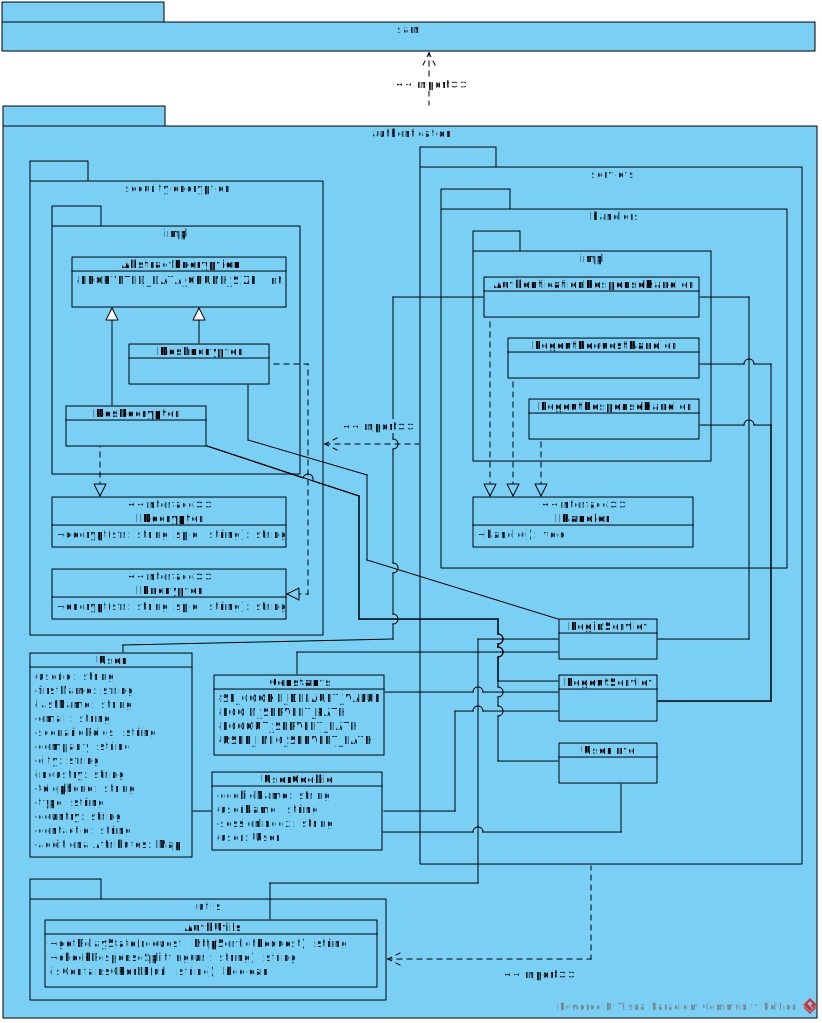
\includegraphics[width=\textwidth]{inc/svg/authenticationModule}
  \caption{Диаграмма классов пакета authentication}
  \label{fig:authenticationModule}
\end{figure}

\begin{figure}
  \centering
  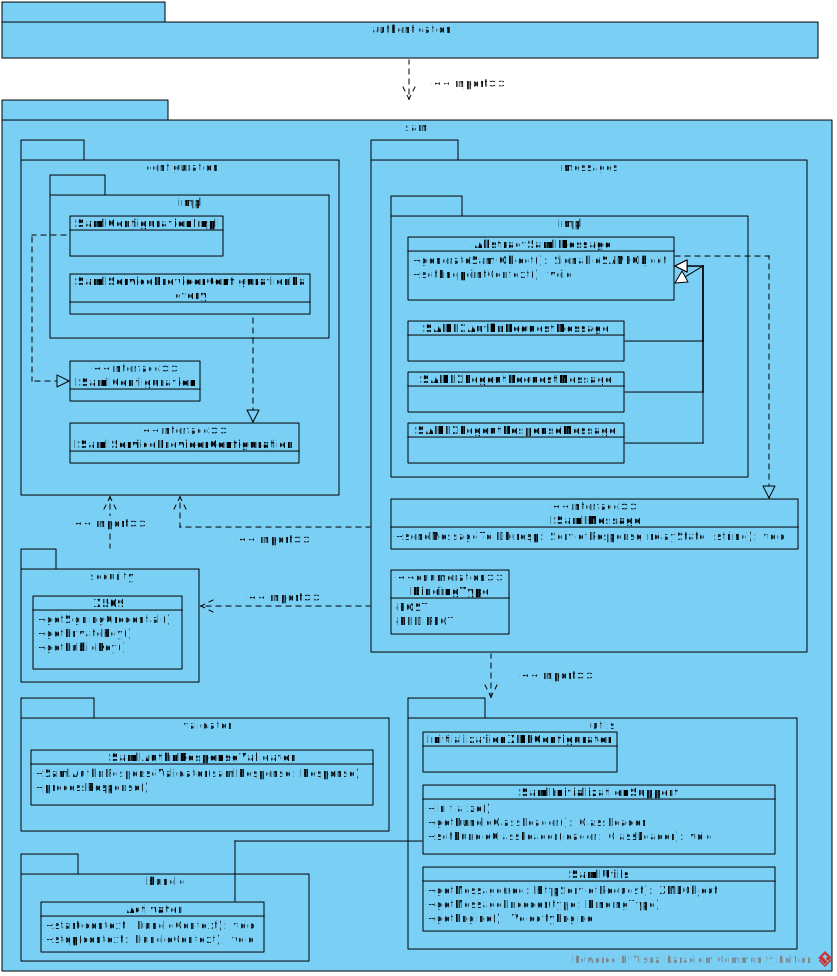
\includegraphics[width=\textwidth]{inc/svg/samlModule}
  \caption{Диаграмма классов пакета saml}
  \label{fig:samlModule}
\end{figure}

%%% Local Variables: 
%%% mode: latex
%%% TeX-master: "rpz"
%%% End: 

%\include{91-appendix2}

\end{document}

%%% Local Variables:
%%% mode: latex
%%% TeX-master: t
%%% End:
